\begin{anexos}
	\begin{figure}[H]
		\centering
		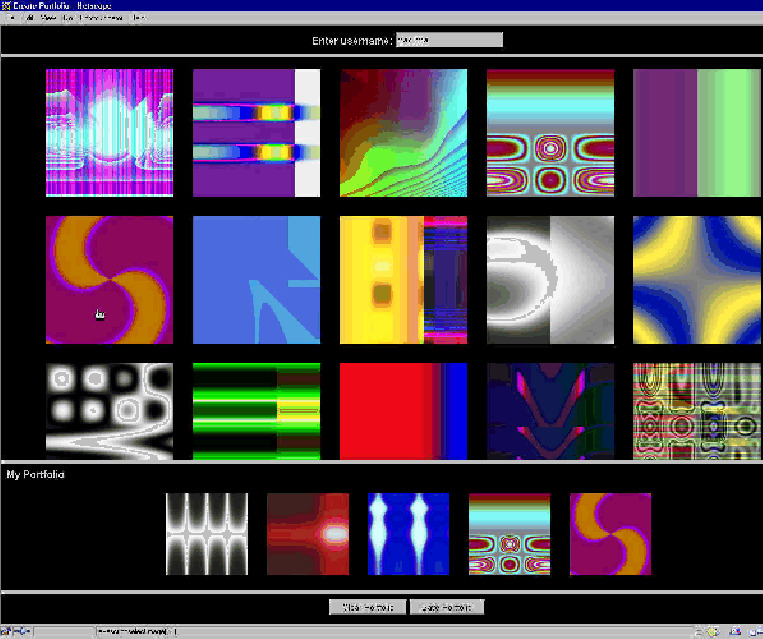
\includegraphics[width=0.5\linewidth]{Deja-Vu.jpg}
		\caption{Selección de portafolio. Fuente: \cite{dhamija2000deja}}
		\label{figure:deja-vu}
	\end{figure}


\begin{figure}[H]
	\centering
	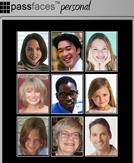
\includegraphics[width=0.3\linewidth]{3.jpg}
	\caption{Sistema PassFaces. Fuente: \cite{inproceedings}}
	\label{passfaces}
\end{figure}

\begin{figure}[H]
	\centering
	\begin{minipage}{0.5\linewidth}  % Tercer cuadrado, 48% del ancho de línea
		\centering
		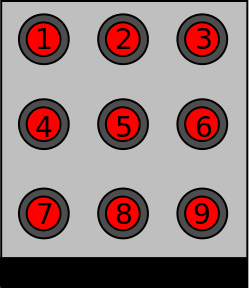
\includegraphics[width=0.7\linewidth]{0.png} % Imagen 3
	\end{minipage}%
	\hfill
	\begin{minipage}{0.5\linewidth} % Cuarto cuadrado, 48% del ancho de línea
		\centering
		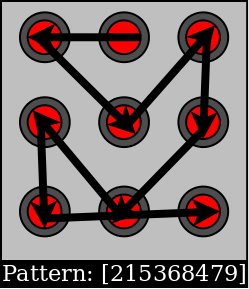
\includegraphics[width=0.7\linewidth]{1.png} % Imagen 4
	\end{minipage}
	\caption{Funcionamiento de un patrón de desbloqueo, Fuente: \cite{aviv2010smudge}}
	\label{android-pattern}
\end{figure}


\begin{figure}[H]
	\begin{minipage}{0.5\linewidth}  % Primer cuadrado, 48% del ancho de línea
		\centering
		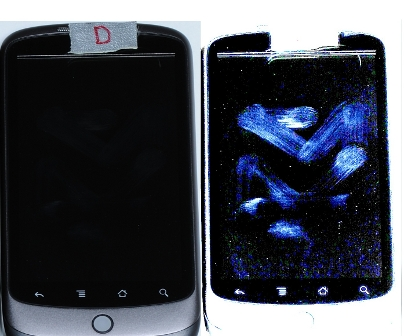
\includegraphics[width=\linewidth]{13.jpg} % Imagen 1
	\end{minipage}%
	\hfill
	\begin{minipage}{0.5\linewidth}  % Segundo cuadrado, 48% del ancho de línea
		\centering
		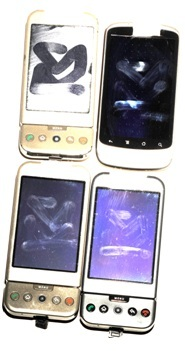
\includegraphics[width=0.5\linewidth]{9.jpg} % Imagen 2
	\end{minipage} % Espacio vertical entre filas

	\caption{Grasa en pantalla usada en los ataques de smudge, Fuente: \cite{aviv2010smudge}}
		\label{smudge-screen}
\end{figure} 

\begin{figure}[H]
	\centering
	\begin{minipage}{0.5\linewidth}  % Tercer cuadrado, 48% del ancho de línea
		\centering
		
\includegraphics[width=0.7\linewidth]{mouse.png} % Imagen 3
		\caption{Dibujado 6 veces usando el mouse, Fuente: \cite{lin2009free}}
		\label{free-draw-train-mouse}
	\end{minipage}%
	\hfill
	\begin{minipage}{0.5\linewidth} % Cuarto cuadrado, 48% del ancho de línea
		\centering
		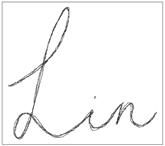
\includegraphics[width=0.7\linewidth]{stylus.png} % Imagen 4
		\caption{Dibujado 6 veces usando stylus, Fuente: \cite{lin2009free}}
		\label{free-draw-train-stylus}
	\end{minipage}
\end{figure}




\begin{figure}[H]
	\centering
	\begin{minipage}{0.48\linewidth}  % Tercer cuadrado, 48% del ancho de línea
		\centering
		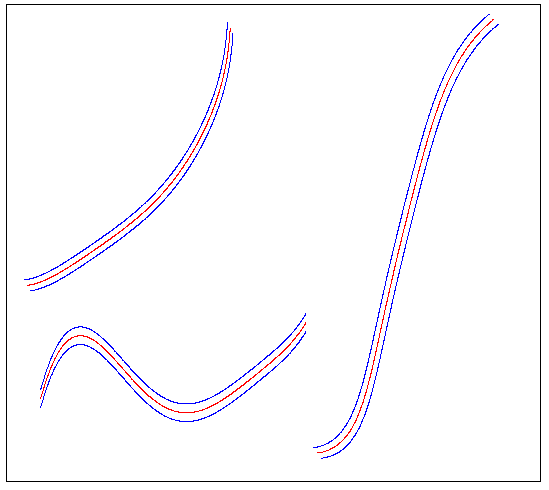
\includegraphics[width=0.9\linewidth]{polinomial.png} % Imagen 3
		\caption{Valores predichos e intervalos de predicción generados por el modelo de regresión polinomial, Fuente: \cite{lin2009free}}
		\label{free-form-draw-polinomial}
	\end{minipage}%
	\hfill
	\begin{minipage}{0.48\linewidth} % Cuarto cuadrado, 48% del ancho de línea
		\centering
		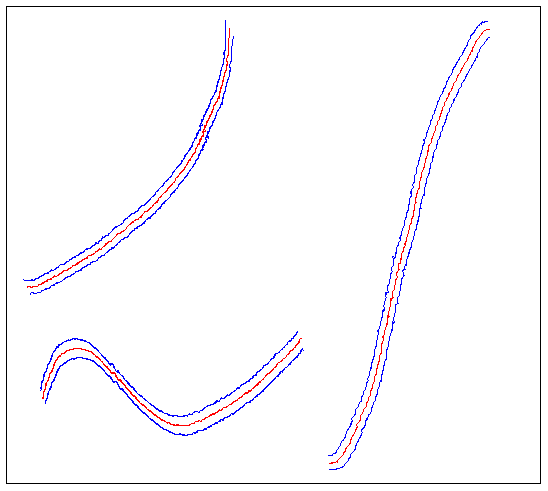
\includegraphics[width=0.9\linewidth]{b-spline.png} % Imagen 4
		\caption{Valores predichos e intervalos de predicción generados por el modelo de regresión B-spline, Fuente: \cite{lin2009free}}
		\label{free-form-draw-spline}
	\end{minipage}
	
\end{figure}


\begin{figure}[H]
	\centering
	\begin{minipage}{0.5\linewidth}  % Tercer cuadrado, 48% del ancho de línea
		\centering
		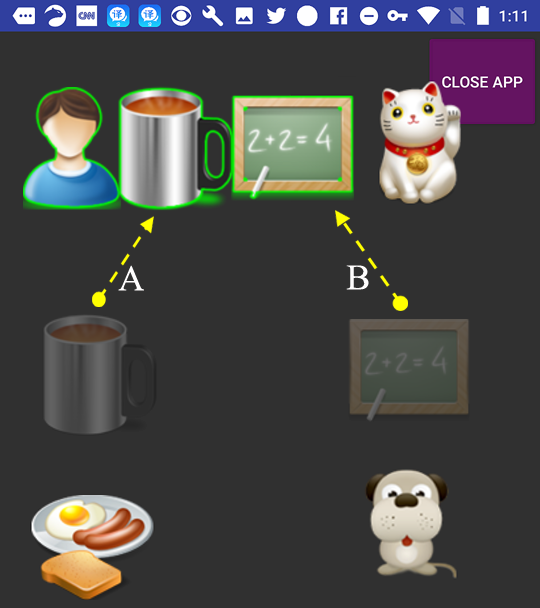
\includegraphics[width=0.8\linewidth]{semantoc-psw-2.png} % Imagen 3
		
	\end{minipage}%
	\hfill
	\begin{minipage}{0.5\linewidth} % Cuarto cuadrado, 48% del ancho de línea
		\centering
		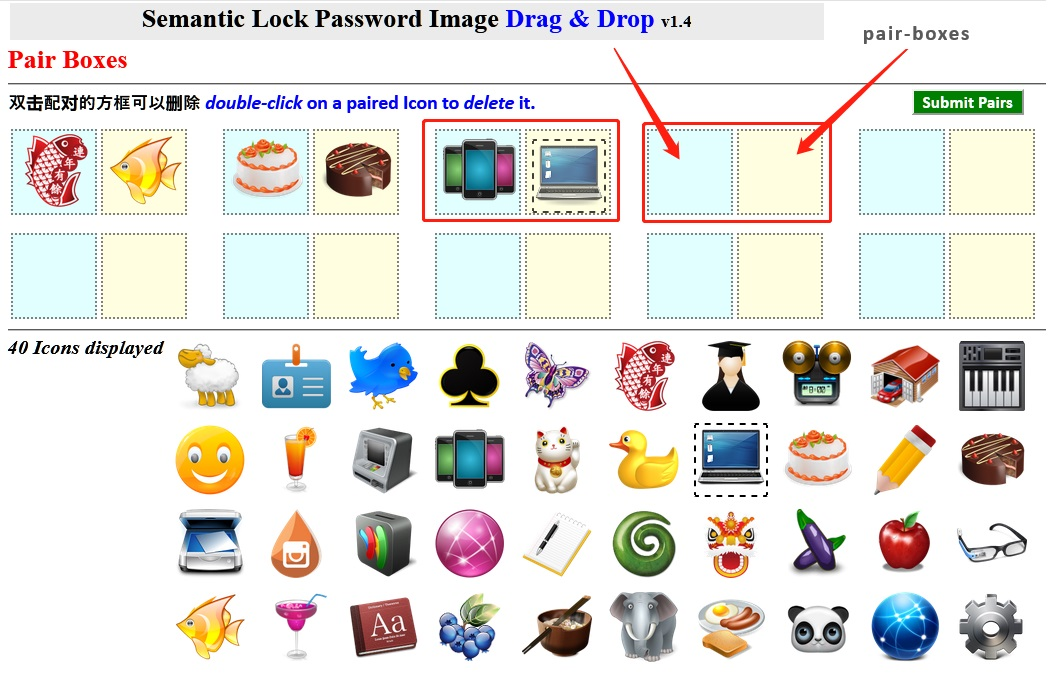
\includegraphics[width=0.8\linewidth]{semantic-psww1.jpg} % Imagen 4
		
	\end{minipage}
	\caption{Funcionamiento de Semantic Lock, Fuente: \cite{olade2023story}}
	\label{semantic-passw}
\end{figure}


\begin{figure}[H]
	\centering
	\begin{minipage}[b]{0.5\linewidth}  % Tercer cuadrado, 48% del ancho de línea
	   \centering
	\adjustbox{valign=b}{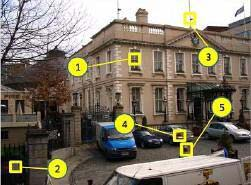
\includegraphics[width=0.8\linewidth]{passpoints.jpg}} % valign=t para alinear la imagen en la parte superior
	\caption{Ejemplo de Passpoints, Fuente: \cite{wiedenbeck2005passpoints}}
	\label{passpoints-example}
	\end{minipage}%
	\hfill
	\begin{minipage}[b]{0.5\linewidth} % Cuarto cuadrado, 48% del ancho de línea
	 \centering
	\adjustbox{valign=b}{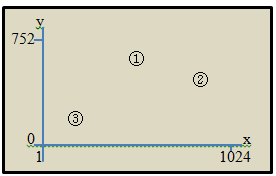
\includegraphics[width=0.8\linewidth]{pass-positions.png}} % valign=t para alinear la imagen en la parte superior
	\caption{Cálculo de hash de un punto Passpositions, Fuente: \cite{8320723}}
	\label{passpositions-example}
	\end{minipage}
	
\end{figure}

\begin{figure}[H]
	\begin{minipage}{0.5\linewidth}  % Primer cuadrado, 48% del ancho de línea
		\centering
		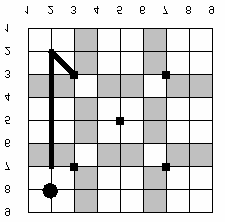
\includegraphics[width=\linewidth]{passgo1.png} % Imagen 1
	\end{minipage}%
	\hfill
	\begin{minipage}{0.5\linewidth}  % Segundo cuadrado, 48% del ancho de línea
		\centering
		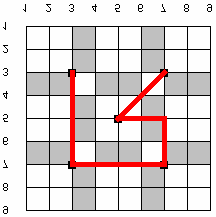
\includegraphics[width=\linewidth]{passgo2.png} % Imagen 2
	\end{minipage} % Espacio vertical entre filas
	\hfill
	\begin{minipage}{0.5\linewidth}  % Segundo cuadrado, 48% del ancho de línea
		\centering
		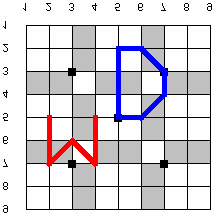
\includegraphics[width=\linewidth]{passgo3.png} % Imagen 2
	\end{minipage} % Espacio vertical entre filas
	\caption{Ejemplos de contraseñas usando Pass Go, Fuente: \cite{tao2008pass}}
	\label{go-passwords}
\end{figure} 

\begin{figure}[H]
	\centering
	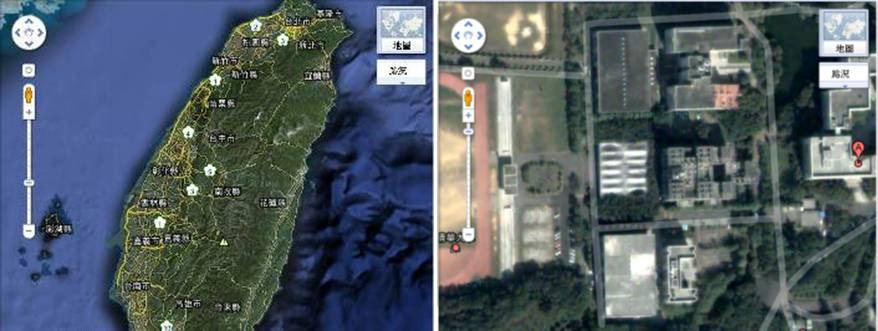
\includegraphics[width=0.5\linewidth]{pass maps2.jpg}
	\caption{Información del mapa en diferentes lugares y niveles de zoom, Fuente: \cite{10.1145/2414456.2414513}}
	\label{passmap}
\end{figure}

\begin{figure}[H]
	\centering
	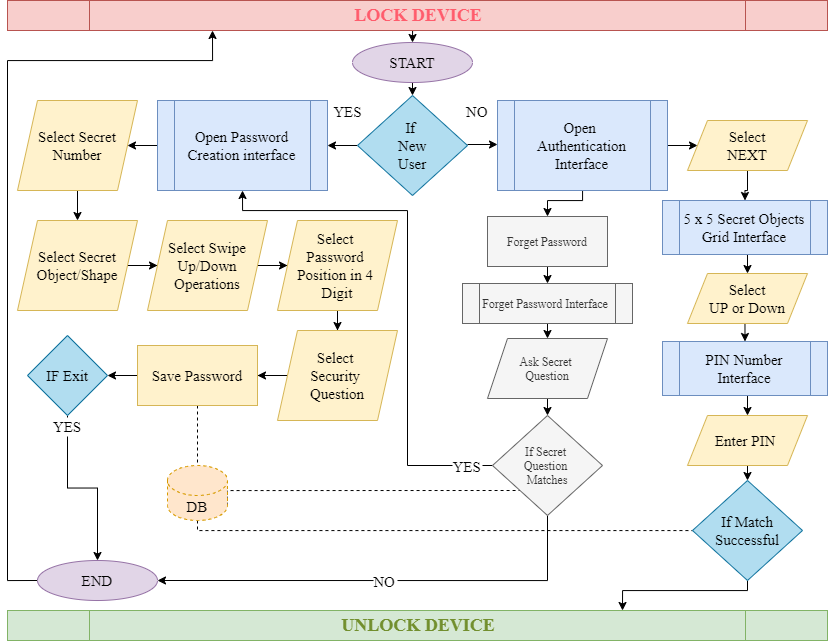
\includegraphics[width=1\linewidth]{grapin-proceso.png}
	\caption{Proceso de autenticación \textit{Gra-Pin}, Fuente: \cite{kausar2022gra} }
	\label{gra-pin}
\end{figure}


 \begin{figure}[H]
	\centering
	\begin{minipage}[b]{0.4\linewidth}  % Tercer cuadrado, 48% del ancho de línea
		\centering
		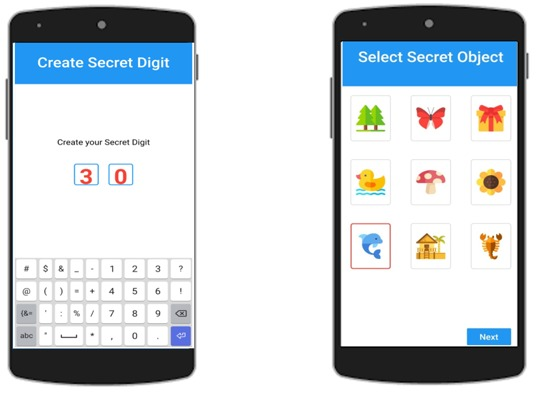
\includegraphics[width=\linewidth]{grapin-secret.jpg}
		\caption{Selección del número e imagen secretos, Fuente: \cite{kausar2022gra} }
	\end{minipage}%
	\hfill
	\begin{minipage}[b]{0.5\linewidth} % Cuarto cuadrado, 48% del ancho de línea
		\centering
		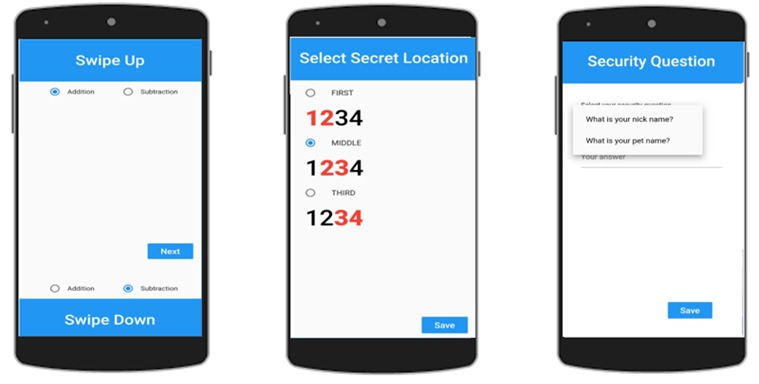
\includegraphics[width=\linewidth]{grapin-position.jpg}
		\caption{Selección de la operación y posición en el Pin de la clave, Fuente: \cite{kausar2022gra}  }          
	\end{minipage}
	\begin{minipage}[b]{0.4\linewidth} % Cuarto cuadrado, 48% del ancho de línea
		\centering
		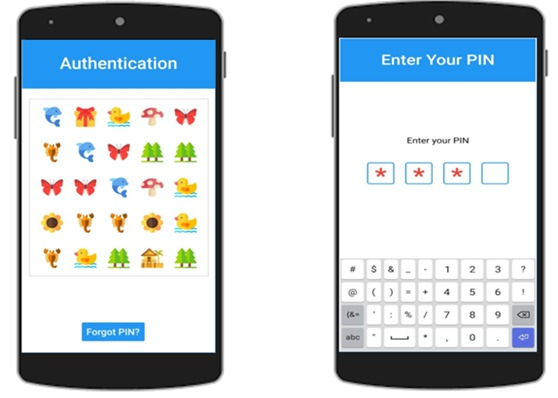
\includegraphics[width=\linewidth]{grapin-auth.jpg}
		\caption{Pantalla de autenticación, Fuente: \cite{kausar2022gra}}
		
	\end{minipage}
	\caption{Pantallas de autenticación de \textit{Gra Pin}, Fuente: \cite{kausar2022gra}}
	\label{gra-pin-screens}
\end{figure}


\end{anexos}
